% Copyright(C) 2011-2015 Pedro H. Penna <pedrohenriquepenna@gmail.com>
%
% This file is part of Nanvix.
%
% Nanvix is free software; you can redistribute it and/or modify
% it under the terms of the GNU General Public License as published by
% the Free Software Foundation; either version 3 of the License, or
% (at your option) any later version.
%
% Nanvix is distributed in the hope that it will be useful,
% but WITHOUT ANY WARRANTY; without even the implied warranty of
% MERCHANTABILITY or FITNESS FOR A PARTICULAR PURPOSE. See the
% GNU General Public License for more details.
%
% You should have received a copy of the GNU General Public License
% along with Nanvix. If not, see <http://www.gnu.org/licenses/>.

\documentclass[10pt,a4paper]{article}

% Input.
\usepackage[utf8]{inputenc}
\usepackage[english]{babel}

% Figures.
\usepackage{graphicx}
\usepackage{subcaption}

% References.
\usepackage[backend=biber]{biblatex}

% Booksmarks.
\usepackage[bookmarks=true,hidelinks]{hyperref}

% Tables.
\usepackage{booktabs}
\usepackage{multirow}
\newcommand{\specialcell}[2][c]%
{\begin{tabular}[#1]{@{}c@{}}#2\end{tabular}}

\author{Pedro H. Penna}
\title{The Nanvix Operating System}

\begin{document}

\maketitle

\section{Introduction}
\label{section: introduction}

% About Nanvix.
Nanvix is an operating system created by Pedro H. Penna for educational purposes. It was designed from scratch to be small and simple, and yet modern and fully featured, so that it could help both, novices and experienced enthusiasts in operating systems, to learn about kernel hacking. The first release of Nanvix came out in early 2011, and since then the system has gone through several changes. This paper details the internals of Nanvix 1.2. All previous and future releases are available at \url{github.com/ppenna/nanvix}, under the GPLv3 license.

% Paper organization.
In this section, we present an overview of Nanvix, starting with the system architecture, then presenting the system services, and finally discussing the required hardware to run the system. In later sections, we present a more detailed description of of Nanvix.

\subsection{System Architecture}
\label{section: system architecture}

% Nanvix and System V.
The architecture of Nanvix is outlined in Figure \ref{figure: nanvix architecture}. It presents a similar structure to Unix System V, and it has been intentionally designed to be so due to two points. First, several successful operating systems, such as Aix, Linux and Solaris, are based on this architecture [??]. Second, System V has earned Dennis Ritchie and Kenneth Thompson the 1983 Turing Award [??]. These points indicate that System V is a well-architected and reliable system, thus serving as a good baseline design for a new educational operating system, such as Nanvix.

% Architecture overview.
Nanvix is structured in two layers. The kernel, the bottom layer, seats on the top of the hardware and runs in privileged mode, with full access to all resources. Its job is to extended the underlying hardware so that: (i) a more pleasant interface, which is easier to program, is exported to the higher level; and (ii) resources can be shared among users, fairly and concurrently. The userland, the top layer, is where all user software run in unprivileged mode, with limited access to the hardware, and the place where the user itself interacts with the system.

% Kernel architecture.
The kernel presents a monolithic architecture, and it is structured in four subsystems: the hardware abstraction layer; the memory management system; the process management system; and the file system. The hardware abstraction layer interacts directly with the hardware and exports to the other subsystems a set of well defined low-level routines, such as those for dealing with IO devices, context switching and interrupt handling. Its job is to isolate, as much as possible, all the hardware intricacies, so that the kernel can be easily ported to other compatible platforms, by simply replacing the hardware abstraction layer.

\begin{figure}[t]
	\centering
	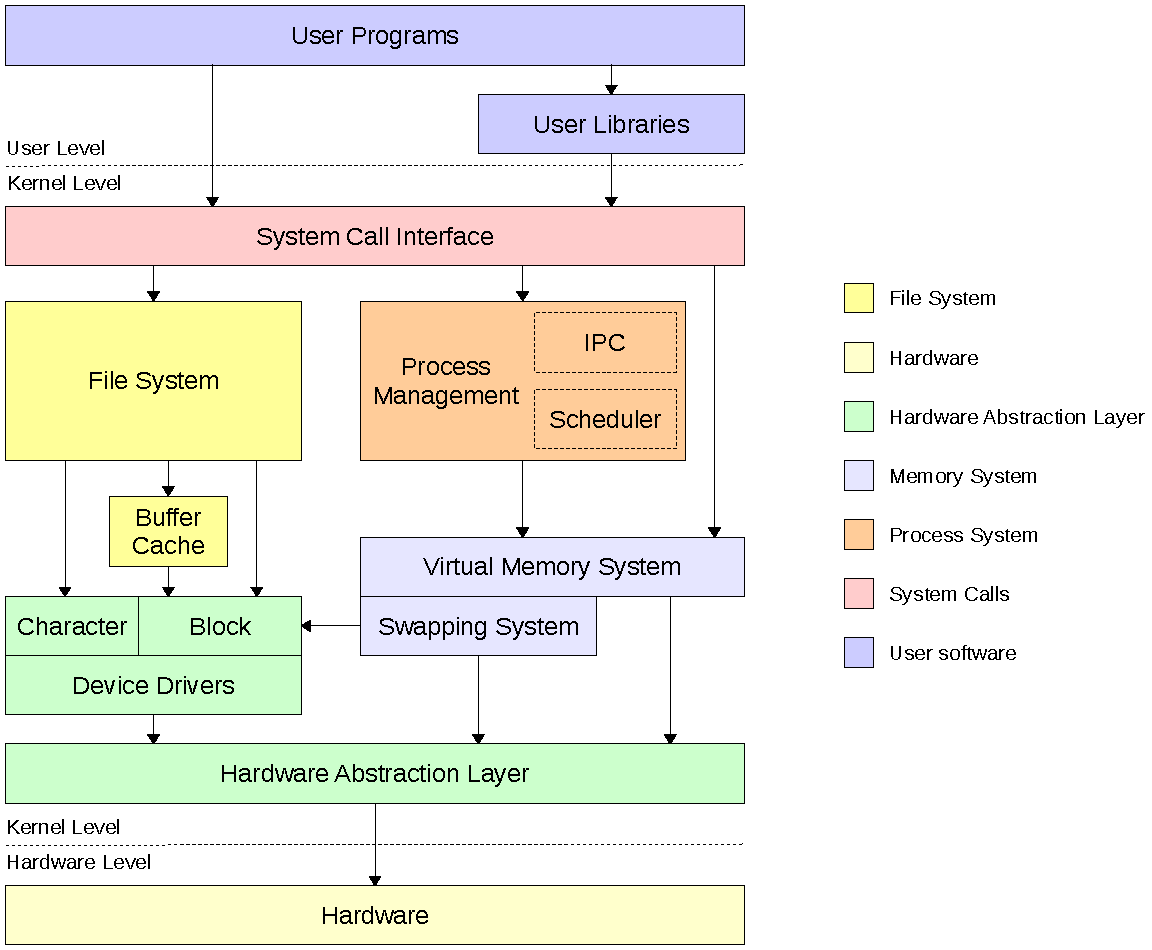
\includegraphics[scale=0.61]{img/nanvix-architecture}
	\caption{Nanvix architecture.}
	\label{figure: nanvix architecture}
\end{figure}

% Memory management system.
The memory management subsystem provides a flat virtual memory abstraction to the system. It does so by having two modules working together: the swapping and virtual memory modules. The swapping module deals with paging, keeping in memory those pages that are more frequently used and swapping out to disk those that are not. The virtual memory system, on the other hand, relies on the paging module to manage higher-level abstractions called memory regions, and thus enable advanced features such as shared memory regions, on-demand loading, lazy coping and memory pinning.

% Process management system.
The process management system handles creation, termination, scheduling, synchronization and communication of processes. Processes are single thread entities and are created on demand, either by the system itself or the user. Scheduling is based on preemption and happens in userland whenever a process runs out of quantum or blocks awaiting for a resource. In kernel land, on the other hand, processes run in nonpreemptive mode and scheduling occurs only when a processes voluntarily relinquishes the processor. Finally, processes many synchronize their activities using semaphores, and communicate with one another through pipes and shared memory regions.

% File system.
The file system provides a uniform interface for dealing with resources. It extends the device driver interface and creates on top of it the file abstraction. Files can be accessed through a unique pathname, and may be shared among several processes transparently.   The file system is compatible with the one present in the Minix 1 operating system, it adopts an hierarchical inode structure, and supports mounting points and disk block caching.

% Userland.
The userland relies on the system calls exported by the kernel. User libraries wrap around some of these calls to provide interfaces that are even more pleasant to programmers. Nanvix offers great support to the Standard C Library and much of the current development effort is focused on enhancing it. User programs are, ultimately, the way in which the user itself interacts with the system. Nanvix is shipped out with the Tiny Shell (\texttt{tsh}) and the Nanvix Utilities (\texttt{nanvix-util}), which heavily resemble traditional Unix utilities. 

\subsection{System Services}
\label{section: system services}

% System calls overview.
The main job of the kernel is to extend the underlying hardware and offer the userland a set of services that are easier to deal with, than those provided by the bare machine. These services are indeed exported as system calls, which user applications invoke just as normal functions and procedures. Nanvix implements 45 system calls, being the majority of them derived from the Posix 1 specification [??]. The most relevant system calls that are present in Nanvix are listed in Table \ref{table: most relevant system calls in nanvix}. In the paragraphs that follow, we briefly discussed each of them. For further information about system calls in Nanvix, refer to the man pages.

% File system system calls: manipulating files.
Files are high-level abstractions created for modeling resources, being primarily designed and used to provide a natural way to manipulate disks. One program that wants to manipulate a file, shall first open it by calling \texttt{open()}. Then, it may call \texttt{read()} and/or \texttt{write()} to read and/or write data to the file. If the file supports random access, the read/write file offset may be moved through the \texttt{lseek()} system call. Finally, when the program is done with that file, it may explicitly close it by calling \texttt{close()}, and have its contents flushed to the underlying device.

% File system system calls: manipulating the file system.
Files are organized hierarchically, in a tree-like structure, and are uniquely identified by their pathnames. Programs may refer to them either by using an absolute pathname, which starts in the root directory; or by using an relative pathname to the current working directory of the program. Programs may change their current working directory by invoking \texttt{chdir()}. Alternatively, users can create links to files by calling \texttt{link()}, and then refer to the linked file by referring to the link (Figure \ref{figure: link system call}). Links and files may be destroyed through the \texttt{unlink()} system call.

\begin{figure}[b]
	\centering
	\begin{subfigure}[b]{0.35\linewidth}
		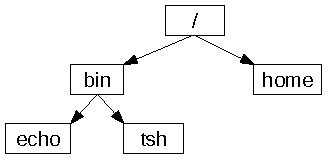
\includegraphics[width=\textwidth]{img/link-1}
		\caption{Before.}
	\end{subfigure} ~ 
	\begin{subfigure}[b]{0.35\linewidth}
		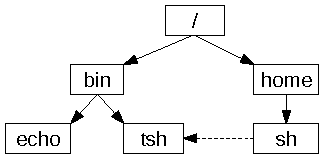
\includegraphics[width=\textwidth]{img/link-2}
		\caption{After.}
	\end{subfigure}
	\caption{\texttt{link()} system call.}
	\label{figure: link system call}
\end{figure}

% File system system calls: file permissions.
Every file has a owner user and a 9-bit flag assigned to it. These flags state what are the read, write and execution permissions for the file, for the owner user, the owner's group users and all others. If a program wants to perform any of these operations it must have enough permissions to do it. The file ownership and permissions may be changed through the \texttt{chown()} and \texttt{chmod()} system calls, respectively, and users can query these information by calling \texttt{stat()}.

% Process management system calls: dealing with processes.
Processes are abstraction of running programs and play a central role in Nanvix. Programs may create new processes by calling \texttt{fork()}, which creates an exact copy of the current running process. The primal process is called the parent and the new process is called child, and they have the same code, stack and data segments, opened files and execution flow, differing only differ in their ID number. Processes may query about their ID by calling \texttt{getpid()} and may change their core through the \texttt{execve()} system call. When the process is done, it invokes \texttt{exit()} to relinquish all resources that it was using.

% Process management system calls: signals and synchronization.
Processes may synchronize their activities using two approaches: through signals or synchronization primitives. In the former, the intend recipient process A first registers a callback function that will handle some specific signal, by calling \texttt{signal()}. If the process has nothing more to do than waiting for a signal to arrive, it may invoke \texttt{pause()} to block until such event happens. Later, another process may send a signal to A by calling \texttt{kill()}, triggering the handler function in A. In the second approach, two processes may open a pipe, a dedicate communication channel, and effectively exchange data with one another. A process in one end of the pipe writes data to it, and in the other end a second processes reads data from the pipe, with the required producer-consumer synchronization being handled by the kernel.

\begin{table}[t]
\small
\centering
\caption{Most relevant system calls that are present in Nanvix.}
\label{table: most relevant system calls in nanvix}
\begin{tabular}{l l l}
	\toprule
	Category & System Call & Description \\
	\midrule
	\multirow{12}{*}{File System}        
	                                     & \texttt{chdir}    & Changes the current working directory           \\
	                                     & \texttt{close}    & Closes a file descriptor                        \\
	                                     & \texttt{chmod}    & Changes the file permissions                    \\
	                                     & \texttt{chown}    & Changes the file ownership                      \\
	                                     & \texttt{ioctl}    & Device control                                  \\
	                                     & \texttt{link}     & Creates a new link to a file                    \\
	                                     & \texttt{lseek}    & Moves the read/write file offset                \\
	                                     & \texttt{open}     & Opens a file descriptor                         \\
	                                     & \texttt{read}     & Reads from a file                               \\
	                                     & \texttt{stat}     & Gets the status of a file                       \\
	                                     & \texttt{unlink}   & Removes a file                                  \\
	                                     & \texttt{write}    & Writes to a file                                \\
	\midrule
	\multirow{7}{*}{\specialcell{Process\\Management}}
	                                     & \texttt{execve}   & Executes a program                              \\
	                                     & \texttt{exit}     & Terminates the current process                  \\
	                                     & \texttt{fork}     & Creates a new process                           \\
	                                     & \texttt{getpid}   & Gets the process ID                             \\
	                                     & \texttt{kill}     & Sends a signal to a process                     \\
	                                     & \texttt{pause}    & Suspends the process until a signal is received \\
	                                     & \texttt{pipe}     & Creates an interprocess communication channel   \\
	                                     & \texttt{signal}   & Signal management                               \\
	\bottomrule
\end{tabular}
\end{table}

\subsection{Hardware Requirements}
\label{section: hardware requirements}

% Target architecture.
Nanvix has been primarily designed to target the x86 architecture. Nevertheless, thanks to the hardware abstraction layer, it may be easily ported to other platforms. Still, the new platform shall meet some requirements to enable this smooth transition.

% Paging.
First, paging shall be somehow supported, since the memory management subsystem relies on this feature to enable virtual memory. Additionally, the hardware shall provide a protection mechanism that would point out whether a page fault has been caused due to a missing page or to a permission violation. Nanvix uses this information to easy the creation of new processes through the copy-on-write technique.

% Interrupts
Second, the hardware shall support interrupts, because Nanvix a preemptive system. More precisely, the hardware shall provide some clock device that would generate interrupts at regular time intervals. The scheduler completely relies on this feature, and the system would not even boot without it, getting stuck on the idle process. Additionally, the hardware should also offer a mechanism to enable and disable interrupts. The kernel uses this to achieve mutual exclusion on critical regions, and thus avoid race conditions.

\section{Process Management}

% Section overview.
In this section, we take a close look in the process management subsystem. We start by first presenting the process structure itself; then highlighting how process scheduling and switching happens; and finally discussing the main mechanisms offered by this subsystem.

\subsection{The Process Structure}
\label{subsection: the process structure}

% Process abstraction overview.
A process is an abstraction of a running program. It depicts the memory core, opened files, execution flow, access permissions, current state and every other relevant information about a program. Table \ref{table: process structure} outlines the (simplified) structure of a process in Nanvix. The information about all processes is kept in a kernel table, named the process table, and it is visible to all subsystems.

\begin{table}[h]
\footnotesize
\centering
\caption{Simplified structure of a process in Nanvix.}
\label{table: process structure}
\begin{tabular}{l l l}
	\toprule
	Category & Field & Description \\
	\midrule
	\multirow{3}{*}{\specialcell{Context Switch\\Information}} & \texttt{kesp}   & Kernel Stack pointer \\
	                                                           & \texttt{kstack} & Kernel Stack         \\
	                                                           & \texttt{intlvl} & Interrupt Level      \\
	\midrule
	\multirow{3}{*}{\specialcell{File System\\Information}} & \texttt{pwd}    & Current Working Directory \\
	                                                        & \texttt{ofiles} & Opened Files              \\	
	                                                        & \texttt{tty}    & Output Terminal Device    \\
	\midrule
	\multirow{2}{*}{\specialcell{General\\Information}} & \texttt{status} & Exit status                                          \\
	                                                    & \texttt{pid}, \texttt{gid}, \texttt{uid} & Process, group and user IDs \\
	\midrule
	\multirow{2}{*}{\specialcell{Memory\\Information}} & \texttt{pregs} & Code, data, stack and heap segment regions \\
	                                                   & \texttt{pgdir} & Page directory       \\
	\midrule
	\multirow{4}{*}{\specialcell{Scheduling\\Information}} & \texttt{state}    & Current state       \\
	                                                       & \texttt{counter}  & Remaining quantum   \\
	                                                       & \texttt{nice}     & Priority adjustment \\	
	                                                       & \texttt{priority} & Priority            \\
	\midrule
	\multirow{2}{*}{\specialcell{Signal\\Information}} & \texttt{received} & Received signals \\
	                                                   & \texttt{handler}  & Signal handlers  \\
	\midrule
	\multirow{2}{*}{\specialcell{Timing\\Information}} & \texttt{utime} & User CPU Time   \\
	                                                   & \texttt{ktime} & Kernel CPU Time \\
	
	\bottomrule
\end{tabular}
\end{table}

% Process table maintenance.
The process management subsystem maintains the process table. Whenever a new process is created, a new entry is added to it; and when a process terminates, its corresponding entry is erased. Nevertheless, each subsystem is in charge of maintaining its own fields in the process structure. For instance, the memory management subsystem is the one that fills up information regarding the segment regions and page directory, whereas the file system keeps track of the current working directory and opened files fields.

% Process states.
A process is created whenever a user launches a program or the system itself spawns a new daemon. After that, the new process goes through a complex lifetime before it terminates, as it is shown in Figure \ref{figure: states of a process in nanvix}.

% State transitions
Initially this new processes is ready to execute (state 1), and it is eventually selected to run by the scheduler. At this moment, the process resumes back its execution in kernel land (state 2) and jumps to userland (state 3). There, the process performs some computation, and it may either gets preempted if it runs out of quantum time (state 4), or gets blocked waiting for a resource (state 5). Either way, the process later resumes its work, and loops back on these states. However, when the process finally gets his job done, or it somehow crashes, it terminates and becomes a zombie process (state 6). A zombie process awaits to gets all resources assigned to it to be taken away by the kernel, and then it is turned to a dead process (state 7).

\begin{figure}[t]
	\centering
	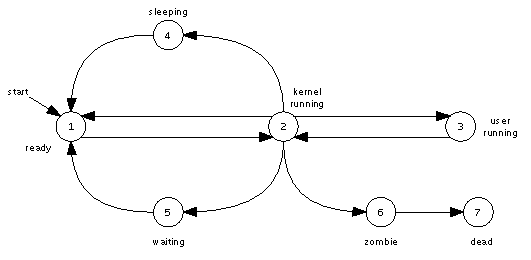
\includegraphics[scale=1.25]{img/process-states}
	\caption{States of a process in Nanvix.}
	\label{figure: states of a process in nanvix}
\end{figure}

\subsection{Process Scheduling and Switching}

% Process scheduling overview.
Several processes may be active in the system, but only one can be running at a time\footnote{Nanvix does not support multiprocessor systems, thus processes are indeed not running in parallel.}. The scheduler chooses which process to run next whenever the running process gets preempted or blocks. In user mode, that happens when the running process runs out of quantum and gets preempted by the kernel, or when it issues a system call. In kernel mode however, scheduling occurs only when the running process voluntarily relinquishes the processor and goes wait for a resource to be released.

% Scheduling policy.
The scheduler uses a priority based criteria to choose the next process to run, with processes with higher priorities being scheduled to run before those with lower priorities\footnote{Nanvix adopts the Unix's priority system style, in which lower values mean higher priorities.}. Processes with equal priorities are chained in a queue and are selected in a round-robin fashion, as it is shown if Figure \ref{figure: scheduler}.

% Priorities of a process.
The priority of a process changes over the time and it is given by the sum of tree numbers: base priority, dynamic priority and nice value. The base priority is assigned by the kernel itself and changes as the process sleeps and wakes up from resource queues, and leaves the kernel or enters it. The dynamic priority is increased by the scheduler as the process waits longer in the ready queue. Finally, the nice value is adjusted by the users, offering them a mechanism to control which processes are more priority over others.

% Process switching.
Once the scheduler choses which process to run next, it performs the context switching operation. It first pushes the contents of all machine registers in the kernel stack. Then, it instructs the memory management unit hardware to switch to the address space of the selected process. Finally, the state of the machine registers are restored from the kernel stack of the selected process. The context switching operation is machine dependent and it is actually carried on by the hardware abstraction layer.

\begin{figure}[t]
	\centering
	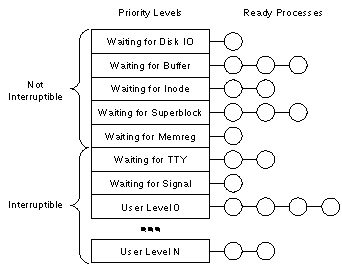
\includegraphics[scale=1.4]{img/scheduler}
	\caption{Scheduler queues.}
	\label{figure: scheduler}
\end{figure}

\subsection{Process Creation and Termination}

% Process creation.
In Nanvix, processes are created through the \texttt{fork()} system call. This call instructs the process management system to create a new process that is an exact copy of the calling process. The primal process is called the parent and the new process is called child, and they have the same code, stack and data segments, opened files and execution flow, differing only differ in their ID number. The \texttt{fork()} system call is a complex and expensive operation, and in order to get it done the process management subsystem heavily interacts with the memory management system and the file system.

% fork() in a nutshell.
First the kernel searches for an empty slot in the process table, to store there all the information about the new process. Then, a new address space for the child process is created: page tables are initialized, the kernel code and data segments are attached to the process' core, and a kernel stack for the process is created. After that, the kernel duplicates every memory region of the parent process and attaches them to the address space of the child process. In this operation, underlying pages are not actually copied, but they are rather linked and copied on demand. This technique, called copy-on-write, greatly speeds up the \texttt{fork()} system call, and it is covered in Section ??. Then, when the address space of the new process is built, file descriptors for all opened files are cloned, and every other information is handcrafted. Finally, the process management system marks the child process as new, so that the scheduler can properly handles this situation, and schedules it in the ready queue for later execution.

% Process termination.
The process then performs some computation and undergoes through a complex lifetime, which we depict in Section \ref{subsection: the process structure}. When the process finally finishes its job it invokes the \texttt{exit()} system call to terminate. This call orders the process management system to actually kill the process and release all resources that are assigned to it.

% exit() in a nutshell.
To do so, several steps are involved. First, the kernel masks out signals and closes all files that are still opened. After that, all child processes of the process that is about to terminate are assigned to a special process, called \texttt{init}\footnote{\texttt{init} is a daemon process whose job is to spawn the logging processes.}. This ensures that no process becomes orphan, and thus become unreachable by signals (see Section ??). Then, the kernel detaches all memory regions from the dying process and marks it as a zombie. At this moment, the dying process still has an address space and a slot in the process table, and it has no way to wipe off these information. The process then hands out this task to the parent process, and sends a death of child (\texttt{SIGCHLD}) to it. This signal cannot be 
blocked or ignored, and it is eventually handled by the corresponding parent process. At this time, the parent process destroys the address space of its zombie child process, and marks the corresponding slot in the process table as not used.

\subsection{Process Communication and Synchronization}

\end{document}